\documentclass[10pt,a4paper]{article}
\usepackage[margin=0.85in]{geometry}
\usepackage{times}
\usepackage{graphicx,booktabs,caption,float}
\usepackage[hyphens]{url}
\urlstyle{rm}
\usepackage[T1]{fontenc}
\captionsetup{font=small,labelfont=bf}
\setlength{\parskip}{3pt}
\setlength{\parindent}{0pt}
\title{\textbf{Can a Small Classifier Pick the Right Disk Scheduler?\\
A Learned Scheduler Selector Under Workload Shift}\\[2pt]
\large CSE-307: Operating Systems, Term Paper (Track 2)}
\author{Mhamuda Shafiq Shamme \quad ID: 202414093 \quad Section B \quad Batch CSE-24}
\date{4 October 2026}
\begin{document}
\maketitle
\vspace{-1.2em}

\section{Problem framing}
Textbooks teach FCFS, SCAN, C-SCAN and SSTF as if you choose one and live with it, but
which one is best really depends on what the requests look like \cite{silberschatz}.
SSTF is greedy and tends to win on seek distance, but it can starve far-away requests \cite{teorey}.
SCAN and C-SCAN are fairer and do well when the queue is full. FCFS is the only one that
costs nothing to run and is fine when the requests already come in track order.
Real machines do not keep one pattern forever, so I wanted to ask a simple question:
\emph{if a small classifier watches a window of incoming requests and picks a scheduler,
does it beat sticking with any single one, and can I trust the confidence number it gives?}

I used a random forest \cite{breiman} from scikit-learn \cite{sklearn}. The test is a timeline
where the workload changes twice, sequential $\rightarrow$ random $\rightarrow$ bursty, which is the
shift the brief asks for. I report total seek distance for each classical scheduler, for the
classifier's choice, and for an oracle that always knows the best one. I also check calibration.

\section{Implementation}
\textbf{Schedulers.} All four are in \texttt{schedulers.py} and return the total head movement
in tracks, with seek time assumed proportional to distance. The disk has 200 cylinders. SCAN and
C-SCAN travel to the disk edge as in the textbook, and the C-SCAN return jump is counted. I
sanity-checked the code on the usual 8-request textbook queue (head at 53): FCFS gives 640,
SSTF 236 and C-SCAN 382, matching the book. SCAN gives 331 because my version sweeps upward
first, while the book's example sweeps downward first (236).

\textbf{Selector.} For each window of 32 pending requests I compute five features: variance
of track positions, mean jump between consecutive requests, fraction of ascending steps,
burstiness (coefficient of variation of the arrival gaps), and how far the centre of the
requests is from the head. A random forest (60 trees, depth 5) predicts the label, which is
the scheduler with the smallest seek total on that window. The confidence is the forest's
highest class probability. The data come from \texttt{make\_dataset.py}: 1200 labelled windows (400 of each workload type), saved as a CSV table with pandas. \texttt{train\_model.py} trains on 70\% of them and tests on the other 30\%. I compared three simple scikit-learn models and a no-model baseline (Table~\ref{tab:models}); the experiment was repeated on 10 freshly generated datasets. I kept the forest because it has the best held-out accuracy and, unlike a single shallow tree, gives many different probability values, which is needed to look at calibration.

\begin{table}[H]
\centering\small
\caption{Held-out comparison of the models (30\% test windows, 10 datasets). ``Extra seek'' is the average seek distance above the best scheduler per window.}
\label{tab:models}
\begin{tabular}{lrr}
\toprule
Model & Accuracy (\%) & Extra seek per window \\
\midrule
Always SSTF (no model) & 65.7 $\pm$ 1.8 & 1.3 $\pm$ 0.2 \\
Decision tree (depth 4) & 71.4 $\pm$ 2.4 & 12.4 $\pm$ 6.5 \\
Logistic regression & 68.0 $\pm$ 2.9 & 11.7 $\pm$ 2.1 \\
Random forest (60 trees) & 73.4 $\pm$ 2.1 & 8.6 $\pm$ 2.8 \\
\bottomrule
\end{tabular}
\end{table}

Note the last column: always choosing SSTF is only right 66\% of the time, yet it loses just 1.3 tracks per window, because when it is wrong the best scheduler is usually only slightly better. The learned models are right more often (up to 73\%) but, when they are wrong, they pick a scheduler that is much worse. Being accurate and having low cost are different things, and Section~\ref{sec:res} shows how this plays out in the timeline test.

\section{Experimental setup}
Three synthetic generators, 32 requests each, head starting at track 100:
\textbf{sequential} (ascending runs with a stride of 1--3 tracks and the odd restart),
\textbf{random} (uniform over all tracks), and \textbf{bursty} (two or three hot spots, requests
come in tight bursts separated by quiet gaps). The classifier is trained on 400 windows of each type.
The test timeline has 60 windows: 20 sequential, then 20 random, then 20 bursty. I repeat it with
30 independent seeds and report mean $\pm$ standard deviation. In a second run the
classifier is trained \emph{without} any bursty windows, to see what happens when the shift
leads to something it has never seen.

\section{Results}\label{sec:res}
\subsection{Seek time}
Table~\ref{tab:seek} gives the numbers and Figure~\ref{fig:seek} the per-phase picture.
Over the whole timeline FCFS is by far the worst (about 56\,000 tracks), SCAN and C-SCAN are in
the middle, and SSTF is the best fixed choice at about 12\,080. The selector reaches
12\,555, which is 78\% less than FCFS, 14\% less than SCAN, and 4.6\% above the oracle (12\,007).
So it does well against most schedulers, but it does \emph{not} beat always using SSTF: it is
about 3.9\% worse.

\begin{table}[H]
\centering\small
\caption{Total seek distance (tracks) over the 60-window timeline, mean $\pm$ s.d.\ of 30 runs.}
\label{tab:seek}
\begin{tabular}{lrrrr}
\toprule
 & Sequential & Random & Bursty & Whole timeline \\
\midrule
FCFS    & 5855 & 42240 & 7942 & 56038 $\pm$ 1357 \\
SCAN    & 4755 & 5849  & 4067 & 14671 $\pm$ 588 \\
C-SCAN  & 6842 & 7831  & 6577 & 21250 $\pm$ 638 \\
SSTF    & 3864 & 5690  & 2527 & 12081 $\pm$ 540 \\
\midrule
Learned & 4013 & 5691  & 2852 & 12555 $\pm$ 580 \\
Oracle  & 3819 & 5662  & 2526 & 12007 $\pm$ 537 \\
\bottomrule
\end{tabular}
\end{table}

\begin{figure}[H]
\centering
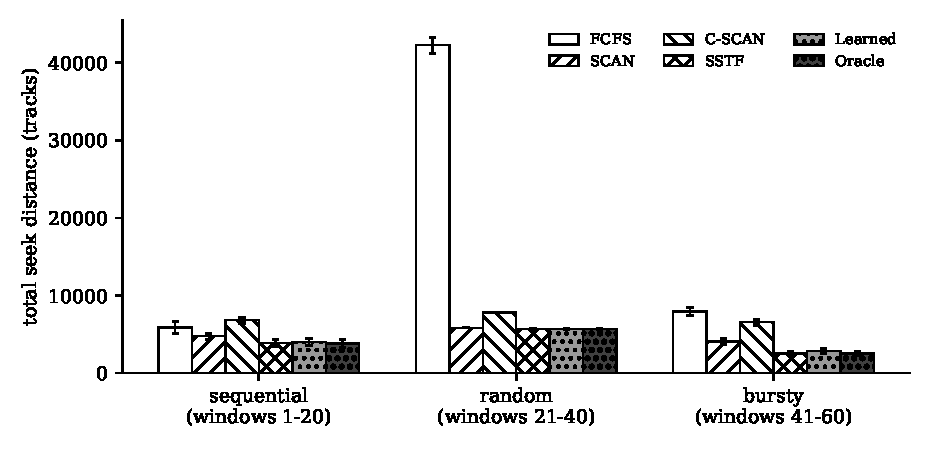
\includegraphics[width=0.82\textwidth]{fig_seek_by_phase.pdf}
\caption{Seek distance per phase of the timeline (error bars: s.d.\ over 30 runs).}
\label{fig:seek}
\end{figure}

\subsection{What changed under the shift}
The shift matters most for FCFS. On the random phase its cost jumps to 42\,240, which is about
seven times the sequential phase, because nothing is reordered and every request is a long jump.
The other three barely notice, since sorting or nearest-first is exactly what you want when the
tracks are scattered. In the bursty phase everything is cheap, since the requests sit close together,
and SSTF gains the most (2527 against 4067 for SCAN): it stays inside a hot spot, while SCAN
still sweeps to the disk edge. C-SCAN pays for its return jump in every phase.

The selector itself is weakest on the sequential phase (62\% correct, against 76\% on random and
79\% on bursty). Looking at the labels, the best scheduler in sequential windows is split
between SSTF (300 of 600), SCAN (187), FCFS (83) and C-SCAN (30), so the classes are close to each other and hard to separate. It is also worth saying that many of the
misses are cheap: an average run makes about 17 wrong picks out of 60, yet the extra cost over
the oracle is only 548 tracks in total, about 33 tracks per miss.

\subsection{Is the confidence calibrated?}
Overall accuracy is $72.2 \pm 5.2$\%. The mean confidence is 0.77 on correct predictions and
0.62 on wrong ones, so the score does carry signal. Figure~\ref{fig:cal} and
Table~\ref{tab:cal} show it is reasonably calibrated: the expected calibration error
\cite{guo} is 0.045. Above 0.84 confidence the classifier is right 96\% of the time, so it is slightly
\emph{under}confident at the top. In the 0.52--0.68 range it is overconfident (mean confidence 0.61,
accuracy 0.49). Using the 0.84 cut-off as a rule (``trust the classifier above it, otherwise fall back to SSTF'') looks
like the sensible way to use the number, but I did not test that rule here.

\begin{figure}[H]
\centering
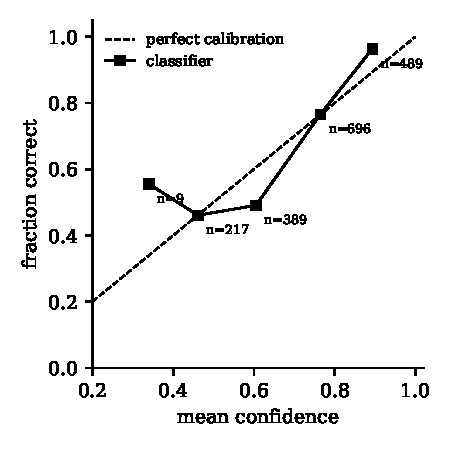
\includegraphics[width=0.40\textwidth]{fig_calibration.pdf}\hspace{1em}
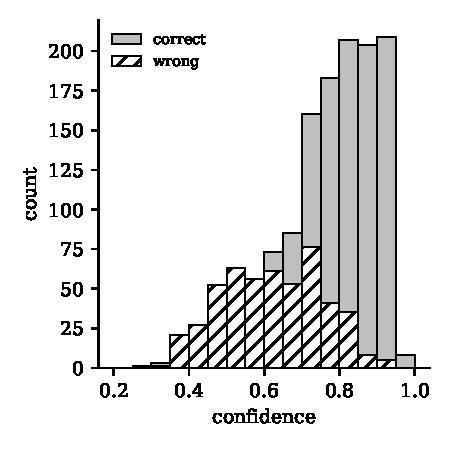
\includegraphics[width=0.40\textwidth]{fig_conf_hist.pdf}
\caption{Left: reliability diagram. Right: confidence of correct and wrong predictions.}
\label{fig:cal}
\end{figure}

\begin{table}[H]
\centering\small
\caption{Calibration by confidence bin (1800 test windows).}
\label{tab:cal}
\begin{tabular}{lrrr}
\toprule
Confidence bin & Windows & Mean confidence & Accuracy \\
\midrule
0.20--0.36 & 9   & 0.34 & 0.56 \\
0.36--0.52 & 217 & 0.46 & 0.46 \\
0.52--0.68 & 389 & 0.61 & 0.49 \\
0.68--0.84 & 696 & 0.76 & 0.77 \\
0.84--1.00 & 489 & 0.89 & 0.96 \\
\bottomrule
\end{tabular}
\end{table}

\subsection{An unseen workload}
When bursty windows are left out of training, the total is 12\,305 $\pm$ 509, accuracy is
70.4\%, and ECE is 0.056. These are almost the same as before, and the total is actually a bit lower. I think this is because the
unseen pattern pushes the forest towards SSTF, the best choice there anyway, rather than because it
generalises well, so I would not read too much into it. The gap between confidence on right and wrong
answers stays (0.73 against 0.62).

\section{Discussion and limits}
The honest summary is that, for \emph{seek distance only}, SSTF is a very strong baseline, and in
my synthetic workloads a classifier that has to choose among four options cannot beat it. The selector earns its keep
mainly by avoiding the bad choices (FCFS on random traffic, C-SCAN everywhere) without being told
the workload type. A selector would matter more under a metric where SSTF suffers, such as
starvation or worst-case wait, which I did not measure. Other limits: windows are treated as one
batch with the head reset to track 100, requests that arrive during service are ignored, the workloads
are synthetic, and the 3.9\% gap to SSTF (about 470 tracks) is smaller than the run-to-run spread of the totals (s.d.\ 540--580), so it
should be read as ``about equal or slightly worse''.

\section{Reproducibility}
Code, raw results and figures are in the GitHub repository at \url{https://github.com/Sham-me09/cse307-disk-scheduler-selector}. Running
\texttt{make\_dataset.py}, \texttt{train\_model.py} and \texttt{run\_experiments.py} in that order regenerates every number here. I used an AI assistant for
help with code and the LaTeX template, as described in the README.

\begin{thebibliography}{9}\small
\bibitem{silberschatz} A.~Silberschatz, P.~B.~Galvin and G.~Gagne, \emph{Operating System Concepts}, 10th ed., Wiley, 2018 (mass-storage structure chapter).
\bibitem{teorey} T.~J.~Teorey and T.~B.~Pinkerton, ``A comparative analysis of disk scheduling policies,'' \emph{Communications of the ACM}, 15(3):177--184, 1972.
\bibitem{breiman} L.~Breiman, ``Random forests,'' \emph{Machine Learning}, 45(1):5--32, 2001.
\bibitem{sklearn} F.~Pedregosa et al., ``Scikit-learn: Machine learning in Python,'' \emph{JMLR}, 12:2825--2830, 2011.
\bibitem{guo} C.~Guo, G.~Pleiss, Y.~Sun and K.~Q.~Weinberger, ``On calibration of modern neural networks,'' in \emph{ICML}, 2017.
\end{thebibliography}
\end{document}
